\section{Exécution \& tests} % (fold)
\label{sec:execution}

Pour ce projet, nous avons effectué des tests de validation sur quelques fonctions, afin de s'assurer que celles-ci marchaient correctement, et pouvoir plus facilement isoler les problèmes. 
De même, le code a été segmenté pour permettre une lecture plus aisée de l'ordre dans lequel s'effectuent les diverses opérations.

\section{Performances} % (fold)
\label{sec:perf}

Les courbes de performances ont été tracées avec gnuplot sur la version \og jouet \fg. 

\begin{figure}[H]
\centering
\verbatiminput{comp_chinois_vol.conf}
\caption{Fichier de configuration utilisé pour les tests}
\label{fig:conf}
\end{figure}
Nous avons utilisé le fichier de configuration de la figure \ref{fig:conf} pour les tests.

Sur la figure \ref{comp_chinois_lin}, on peut voir qu'avec le vol de tâche, on peut être beaucoup plus rapide qu'en attribuant les tâches de manière statique aux différents processus. En effet, pour la version multithreadé, nous ne faisions qu'attribuer des tâches d'une longueur définie à un certain processus, et celui-ci les parallélisait ensuite parmi ses threads. Ainsi, les processus ayant les tâches les plus longues, pourtant bien moins nombreuses. Sur cet exemple, nous affections 10 tâches de longueur 5e+6 $\mu s$ au Processeur 1.
\begin{figure}[H]
\centering
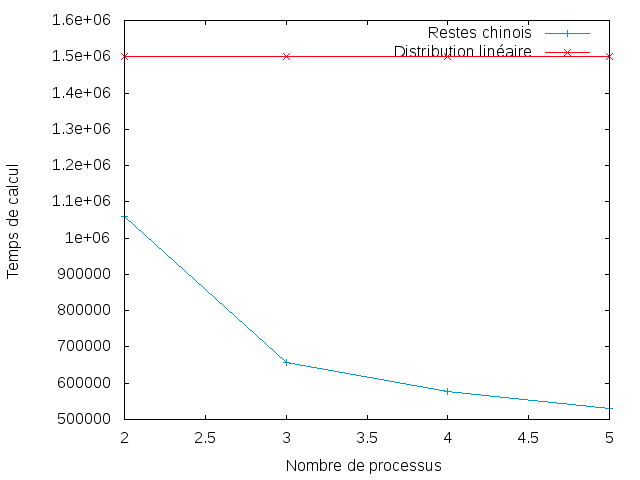
\includegraphics[width=0.8\textwidth]{comp_chinois_lin.png}
\caption{Le vol de tâche permet d'être plus rapide}
\label{comp_chinois_lin}
\end{figure}
On peut voir sur la figure \ref{comp_chinois_vol} que le vol de travail avec une distribution linéaire est plus intéressant que d'utiliser les restes chinois pour avoir une distribution pseudo aléatoire, sans utiliser le vol de travail.
\begin{figure}[H]
\centering
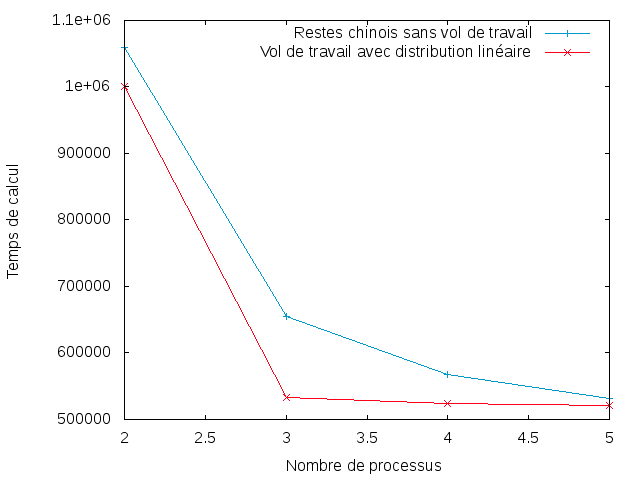
\includegraphics[width=0.8\textwidth]{comp_chinois_vol.png}
\caption{Le vol de tâche permet d'être plus rapide}
\label{comp_chinois_vol}
\end{figure}
% section \ (end)
